

%-------------------------------------------------------------------------------
% Dokumenten Klasse
\documentclass[
	final,
	a4paper,
	oneside,
	parskip=full,
	headings=standardclasses,
	headings=big,
	pointednumbers
]{scrartcl}

%-------------------------------------------------------------------------------
% Packete nutzen
\usepackage[T1]{fontenc}
\usepackage[utf8]{inputenc}
\usepackage[left=20mm,right=25mm,top=20mm,bottom=25mm]{geometry}
\usepackage{amsmath}
\usepackage{amssymb}
\usepackage{mathtools}
\usepackage{mathtools}

%-------------------------------------------------------------------------------
% xcolor
\usepackage[svgnames]{xcolor}

%-------------------------------------------------------------------------------
% TikZ
\usepackage{tikz}
\usetikzlibrary{positioning, arrows, decorations, calc}

%-------------------------------------------------------------------------------
% 
\newcommand{\f}[2]{\frac{#1}{#2}}
\newcommand{\fs}[2]{{\tfrac{#1}{#2}}}

% kl = ()
\newcommand{\kl}[1]{{\left( #1 \right)}}

% kq = {}
\newcommand{\kq}[1]{{\left\{ #1 \right\}}}

% ks = []
\newcommand{\ks}[1]{{\left[ #1 \right]}}

\begin{document}

    \begin{tabular}{ccc}
        Polygon & Bounding Box & Triangles Removed \\
        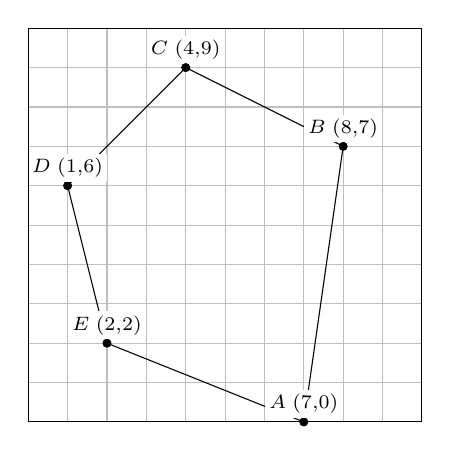
\begin{tikzpicture}[]
            \def\xlines{10}
            \def\ylines{10}
            \def\raster{5mm}
    
            \coordinate (A) at (7*\raster,0*\raster);
            \coordinate (B) at (8*\raster,7*\raster);
            \coordinate (C) at (4*\raster,9*\raster);
            \coordinate (D) at (1*\raster,6*\raster);
            \coordinate (E) at (2*\raster,2*\raster);
    
            % draw vertical lines
            \foreach \x in {0,...,\xlines}
            {
                \draw[lightgray] (\x * \raster, 0mm) -- (\x * \raster, \ylines * \raster);
            }
    
            % draw horizontal lines
            \foreach \y in {0,...,\ylines}
            {
                \draw[lightgray] (0mm, \y * \raster) -- (\xlines * \raster, \y * \raster);
            }

            \draw
                (A) -- (B) -- (C) -- (D) -- (E) -- (A); 
            
            \foreach \point/\a/\b/\i in {A/7/0/1,B/8/7/2,C/4/9/3,D/1/6/4,E/2/2/5}{
                \draw[black,fill=black]
                    let \p1 = (\point)
                    in (\x1, \y1) circle (0.5mm);
                \path
                    let \p1 = (\point)
                    in
                        node[above, fill=white, inner sep=1.5, outer sep=1.5] at (\x1, \y1) {$\scriptstyle \point \; \left( \a, \b \right) $};
            }
            
    
            % border
            \draw[black] (0mm, 0mm) -- (\xlines * \raster, 0mm);
            \draw[black] (0mm, 0mm) -- (0mm, \ylines * \raster);
            \draw[black] (\xlines * \raster, 0mm) -- (\xlines * \raster, \ylines * \raster);
            \draw[black] (0mm, \ylines * \raster) -- (\xlines * \raster, \ylines * \raster);
        \end{tikzpicture} &
        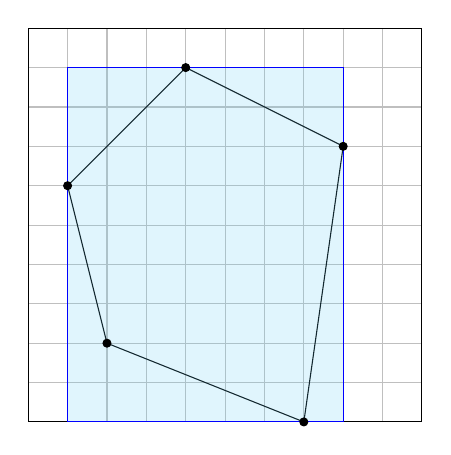
\begin{tikzpicture}[]
            \def\xlines{10}
            \def\ylines{10}
            \def\raster{5mm}
    
            \coordinate (A) at (7*\raster,0*\raster);
            \coordinate (B) at (8*\raster,7*\raster);
            \coordinate (C) at (4*\raster,9*\raster);
            \coordinate (D) at (1*\raster,6*\raster);
            \coordinate (E) at (2*\raster,2*\raster);

            % draw vertical lines
            \foreach \x in {0,...,\xlines}
            {
                \draw[lightgray] (\x * \raster, 0mm) -- (\x * \raster, \ylines * \raster);
            }
    
            % draw horizontal lines
            \foreach \y in {0,...,\ylines}
            {
                \draw[lightgray] (0mm, \y * \raster) -- (\xlines * \raster, \y * \raster);
            }
            
            % border
            \draw[black] (0mm, 0mm) -- (\xlines * \raster, 0mm);
            \draw[black] (0mm, 0mm) -- (0mm, \ylines * \raster);
            \draw[black] (\xlines * \raster, 0mm) -- (\xlines * \raster, \ylines * \raster);
            \draw[black] (0mm, \ylines * \raster) -- (\xlines * \raster, \ylines * \raster);
            
            \draw
                (A) -- (B) -- (C) -- (D) -- (E) -- (A); 

            \draw[blue, fill=cyan!60, fill opacity=0.2]
                (1*\raster, 0*\raster) rectangle (8*\raster, 9*\raster);
    
            \foreach \point/\a/\b in {A/7/0,B/8/7,C/4/9,D/1/6,E/2/2}{
                \draw[black,fill=black]
                    let \p1 = (\point)
                    in (\x1, \y1) circle (0.5mm);
            }
        \end{tikzpicture} &
        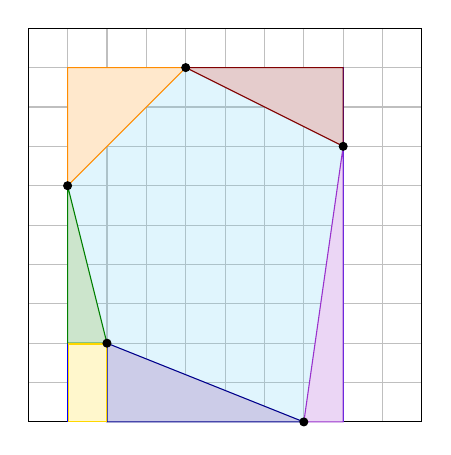
\begin{tikzpicture}[]
            \def\xlines{10}
            \def\ylines{10}
            \def\raster{5mm}
    
            \coordinate (A) at (7*\raster,0*\raster);
            \coordinate (B) at (8*\raster,7*\raster);
            \coordinate (C) at (4*\raster,9*\raster);
            \coordinate (D) at (1*\raster,6*\raster);
            \coordinate (E) at (2*\raster,2*\raster);
            
    
            % draw vertical lines
            \foreach \x in {0,...,\xlines}
            {
                \draw[lightgray] (\x * \raster, 0mm) -- (\x * \raster, \ylines * \raster);
            }
    
            % draw horizontal lines
            \foreach \y in {0,...,\ylines}
            {
                \draw[lightgray] (0mm, \y * \raster) -- (\xlines * \raster, \y * \raster);
            }
            
            % border
            \draw[black] (0mm, 0mm) -- (\xlines * \raster, 0mm);
            \draw[black] (0mm, 0mm) -- (0mm, \ylines * \raster);
            \draw[black] (\xlines * \raster, 0mm) -- (\xlines * \raster, \ylines * \raster);
            \draw[black] (0mm, \ylines * \raster) -- (\xlines * \raster, \ylines * \raster);
    
            \draw[blue, fill=cyan!60, fill opacity=0.2]
                (1*\raster, 0*\raster) rectangle (8*\raster, 9*\raster);
    
            \draw[Green, fill=Green!20]
                (D) -- (E) -- (1*\raster, 2*\raster) -- (D);
            \draw[DarkOrange, fill=DarkOrange!20]
                (C) -- (D) -- (1*\raster, 9*\raster) -- (C);
            \draw[Maroon, fill=Maroon!20]
                (B) -- (C) -- (8*\raster, 9*\raster) -- (B);
            \draw[DarkOrchid, fill=DarkOrchid!20]
                (A) -- (B) -- (8*\raster, 0*\raster) -- (A);
            \draw[DarkBlue, fill=DarkBlue!20]
                (E) -- (A) -- (2*\raster, 0*\raster) -- (E);
            \draw[Gold, fill=Gold!20]
                (1*\raster + 0.1mm, 0*\raster + 0.1mm) rectangle (2*\raster - 0.1mm, 2*\raster - 0.1mm);
    
            \foreach \point/\a/\b in {A/7/0,B/8/7,C/4/9,D/1/6,E/2/2}{
                \draw[black,fill=black]
                    let \p1 = (\point)
                    in (\x1, \y1) circle (0.5mm);
            }
        \end{tikzpicture} \\
        {$\!\begin{aligned}[t]
            A = \f{1}{2} \sum_{i=1}^n (y_i + y_{i+1})(x_i - x_{i+1}) \\
        \end{aligned}
        $} &
        {$\!\begin{aligned}[t]
            A_{BB} = 7 \cdot 9 \\
        \end{aligned}
        $} &
        {$\!\begin{aligned}[t]
            A = A_{BB} - \sum_{i=1}^n A_{R_i} \\
        \end{aligned}
        $} \\
        {$\!\begin{aligned}[t]
            \\
            \arraycolsep=1.4pt
            \begin{array}{rllll}
                \f{1}{2} \left[ \right. & \kl{0+7} & \cdot & \kl{7-8} & + \\
                                        & \kl{7+9} & \cdot & \kl{8-4} & + \\
                                        & \kl{9+6} & \cdot & \kl{4-1} & + \\
                                        & \kl{6+2} & \cdot & \kl{1-2} & + \\
                                        & \kl{2-0} & \cdot & \kl{2-7} & \left. \right]= 42 \\
            \end{array}
        \end{aligned}
        $} & &
        {$\!\begin{aligned}[t]
            \\
            \arraycolsep=1.4pt
            \begin{array}{rlll}
                7 \cdot 9 & - & \f{1 \cdot 7}{2} & - \\
                          &   & \f{4 \cdot 2}{2} & - \\
                          &   & \f{3 \cdot 3}{2} & - \\
                          &   & \f{4 \cdot 1}{2} & - \\
                          &   & \f{5 \cdot 2}{2} & - \\
                          &   & 2 \cdot 1        & = 42 \\
            \end{array}
        \end{aligned}
        $}
    \end{tabular}


\end{document}